\chapter{Particle reconstruction}
\label{chap:objectReco}

\section{Introduction}

To extract a potential \Hee signal, a fit is performed to the dielectron invariant mass distribution in each constructed analysis category. For \Hee signal events, the \mee distribution forms a narrow peak centred close to the value of the Higgs boson mass, sitting on top of a smoothly falling background from SM processes other than the \Hee decay. For events with two electrons, $e_{1}$ and $e_{2}$, under the approximation of negligible electron mass, the dielectron invariant mass is given by the expression:

\begin{equation}\label{eqn:hee_mee}
    m_{ee} = \sqrt{2E_{e_1}E_{e_2}(1-\cos{\theta})},
\end{equation}


\noindent where $E_{e_1}$ and $E_{e_1}$ are the energies of the leading and subleading-\Et electron respectively, and $\theta$ is the opening angle between them. In order to resolve the signal peak resulting from \Hee decays over the background continuum, Eqn~\ref{eqn:hee_mee} demonstrates that both the electron energies and directions, as well as the position of the primary interaction vertex, must be well measured. Since the analysis sensitivity depends on the signal-to-background ratio, $S/B$, electrons from the \Hee decay must also be correctly identified against those resulting from background processes. 

This chapter firstly outlines the simulated samples and data used within the event categorisation and to produce the analysis' results. The remainder of the chapter describes the reconstruction of physics objects at CMS, many of which are used within the \Hee search, and the corrections applied to them. A particular focus is placed on the reconstruction of electrons, including the per-electron identification techniques. Additional suppression of background events at the per-event level is also discussed in chapter~\ref{chap:eventCategorisation}. 

\section{Samples}

\subsection{Data}

This search uses 138~fb$^{-1}$ of pp collision data collected by the CMS experiment at \sqrts~TeV, of which 36.3, 41.5, and 59.8~\fbinv were collected during 2016, 2017, and 2018, respectively.
Data is selected using the two-tiered trigger system at CMS. 
%Although the CMS trigger menu\cite{HLT} includes dedicated single electron and dielectron HLT paths, triggers targeting single electrons typically require tighter \Et requirements in order to maintain a tolerable event rate. This results in a reduction in the efficiency of selecting $\Hee$ events with lower \pt, and therefore only dielectron triggers (with asymmetric \pt thresholds) are used in the analysis.
%also our offline selection is as tight as single electron thresholds and so wouldn't even gain by doing or OR or the two
The analysis uses a dedicated dielectron HLT path, which requires each electron to be seeded by at least one EM candidate in the L1T. For data taken in 2016, seeds were required to have a minimum transverse energy of 23 and 10~GeV for the leading and subleading electron respectively. For 2017 and 2018, the requirements were increased to 25 and 14~GeV respectively~\cite{CMS_egamma_performance}.
In the HLT, energy deposits associated with the L1T seeds are clustered using a procedure similar to the offline algorithm. Electron candidates are then selected based on properties of the resulting supercluster. For triggers targeting dielectron objects, this selection is similar to that of the L1T, and includes thresholds of 23~GeV and 12~GeV on the leading and subleading electron respectively.
Requirements are also placed on the shower shape and isolation properties of the cluster. 
This includes selection on the root-mean-square of the shower width in $\eta$, which describes the lateral shower profile.
The isolation requirement limits contributions from energy deposits outside of a cone with axis centred on the EM candidate, with radius $\Delta R=0.3$, to be less than 20\% of the cluster \Et.
%For electrons with $|\eta|<1.479$, a threshold of $\sigma_{i\eta i\eta} \leq0.013$ is applied, while for electrons with $1.479 < |\eta|<2.65$, the requirement is loosened to $\sigma_{i\eta i\eta} \leq 0.035$. 
%The isolation requirements are 0.2 * E_{T}

The efficiency of the trigger is evaluated in Drell-Yan (DY) \Zee events in a control region around the $\mathrm{Z}$ boson mass.
Drell-Yan events are chosen since a relatively pure sample of electrons that are kinematically similar to those from the \Hee decay can be obtained.
Trigger efficiencies are measured using the tag-and-probe~\cite{TagAndProbe} method.  
This method selects one electron, named the \textit{tag}, which satisfies tight electron identification and isolation requirements. A second electron, named the \textit{probe}, is then chosen to pass a criteria specific to the efficiency being measured --- in this case, the dielectron HLT requirements.
The efficiency is measured in both data and simulated samples, with the ratio being used to correct simulation to data.
The set of corrections are derived differentially in bins of supercluster \pt and $\eta$, independently for each era of data taking.
Figure~\ref{fig:hee_trigger_sfs} shows the resulting scale factor distributions, where for all eras, the corrections are close to unity.



\begin{figure}[htbp!]                                        
\centering                                                   
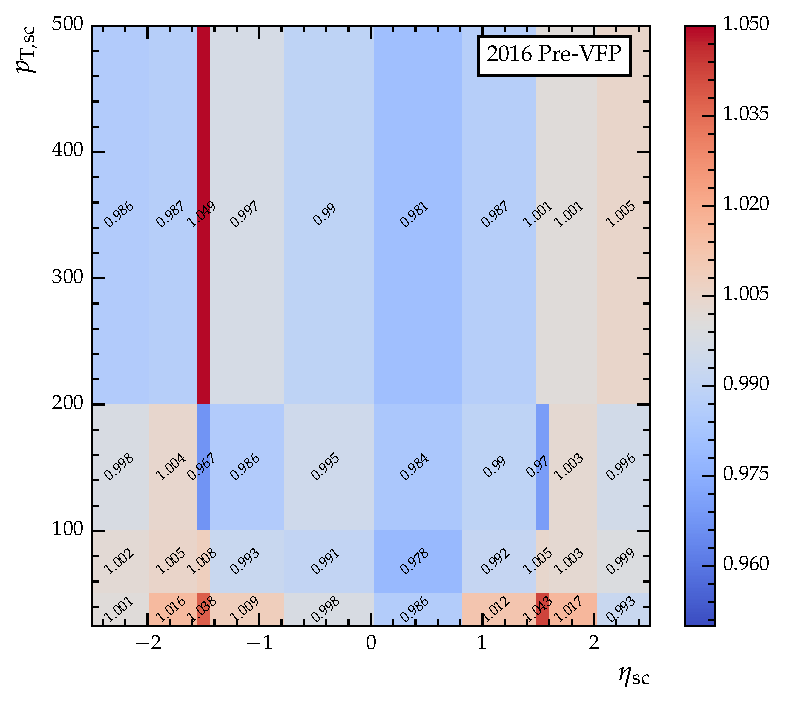
\includegraphics[width=0.48\linewidth]{Figures/Hee/simulationCorrections/TriggerSFs/Trigger_SFs_2016PreVFP.pdf}\hfill
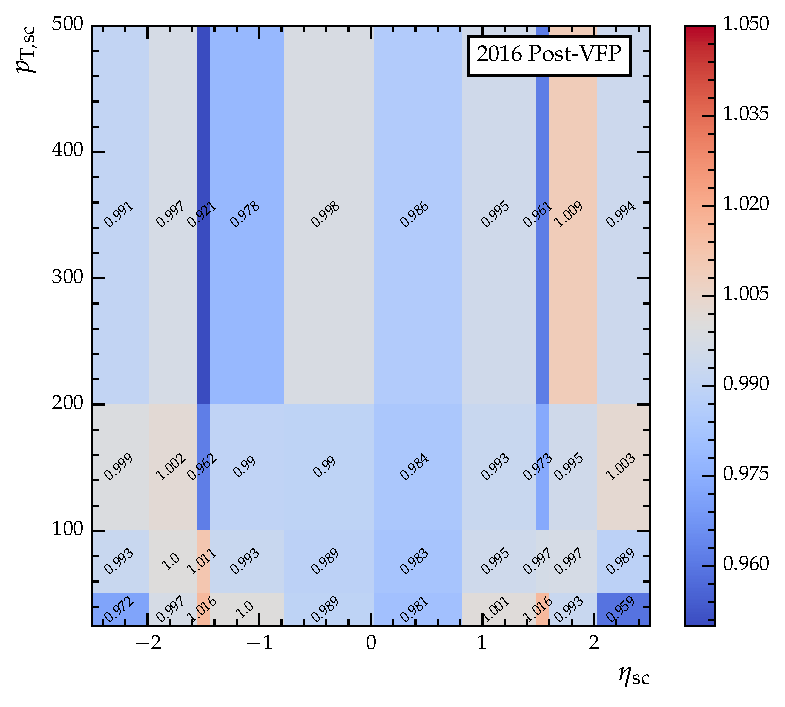
\includegraphics[width =0.48\linewidth]{Figures/Hee/simulationCorrections/TriggerSFs/Trigger_SFs_2016PostVFP.pdf}\hfill%
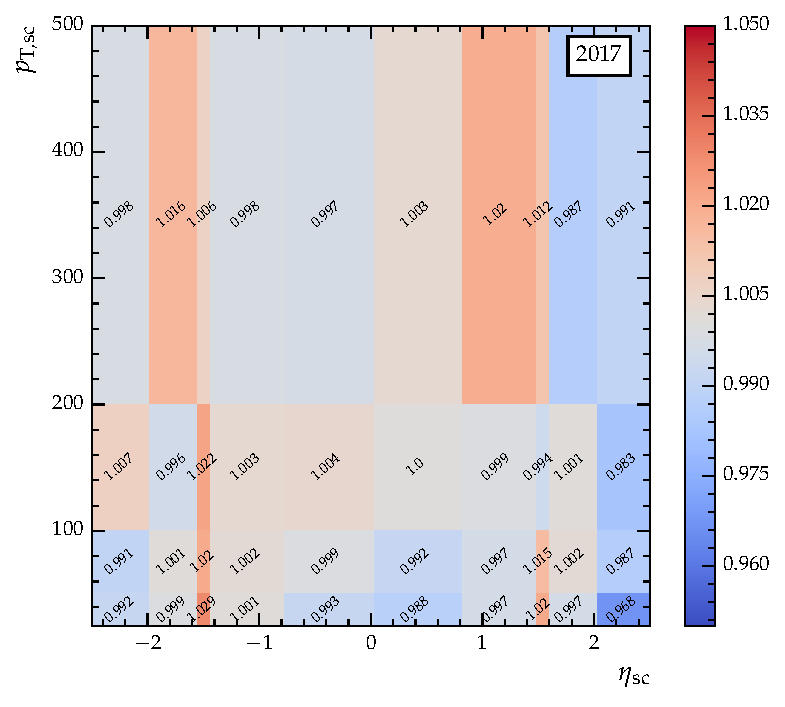
\includegraphics[,width =0.48\linewidth]{Figures/Hee/simulationCorrections/TriggerSFs/Trigger_SFs_2017.pdf}\hfill
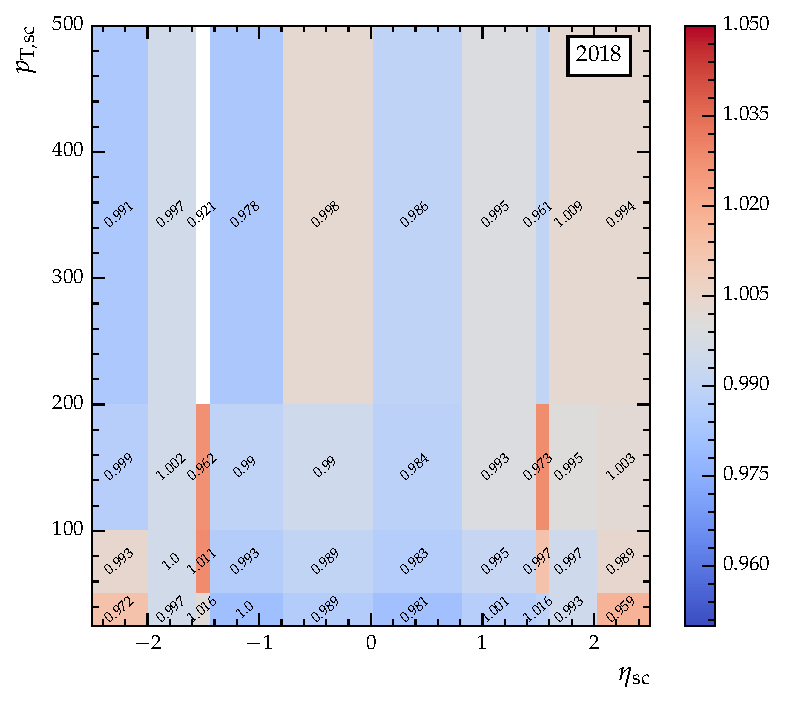
\includegraphics[width =0.48\linewidth]{Figures/Hee/simulationCorrections/TriggerSFs/Trigger_SFs_2018.pdf}\hfill%

\caption[Trigger efficiencies for data and simulated samples.]{Ratio of trigger efficiencies for data and simulation as a joint function of supercluster \pt and $\eta$, for 2016, 2017, and 2018. Corrections are evaluated in a sample of \Zee events using the tag-and-probe method, before being applied to simulation. Note that two independent sets of corrections are derived for samples in 2016, to account for changing conditions in the mitigation of highly ionising particles.}
\label{fig:hee_trigger_sfs}                                 
\end{figure} 

\subsection{Simulation}

In this analysis, simulated samples produced using Monte Carlo (MC) techniques are used to model signal events and train MVA-based event classifiers. Simulated signal samples are produced for the four Higgs boson production modes with the highest cross sections at the LHC, including ggH, VBF, VH, and ttH events. The matrix element (ME) for each process is calculated using the \textsc{Madgraph5\_}a\textsc{mc@nlo} v2.6.5~\cite{madgraph5} package at next-to-leading order accuracy in perturbative QCD. The resulting parton-level samples are then interfaced with \textsc{pythia}~v8.230~\cite{pythia8} which simulates the parton showering and hadronisation processes, using the CP5 underlying event tune~\cite{CP5Tune} to calibrate soft QCD processes. %TUNE: Soft scattering processes cannot be described by perturbative QCD. Hence we need to measure these interactions in data and \textbf{tune} a model to what we observe. We do this each time our collision condition change. Underlying event means everything not associated with the hard scattering event, that can still interact with the hard process. 
The yield of each signal sample is normalised by the corresponding Higgs boson production cross section~\cite{YR4}, the \Hee branching fraction, and the acceptance of the analysis preselection.

The largest fraction of background events originate from Drell-Yan processes, where the $\mathrm{Z}$ boson decays to two electrons. Smaller contributions from \ttbar processes are also present, where each top quark in the pair decay via a $\mathrm{W}$ boson. These decays are divided into a dilepton mode, where both $\mathrm{W}$ bosons decay to a lepton and associated neutrino, and a semi-leptonic mode where one $\mathrm{W}$ boson decays hadronically, with the corresponding jet misidentified as an electron. Since the electron misidentifaction rate is low, semi-leptonic \ttbar decays account only for a very small fraction of background events. Finally, processes where a $\mathrm{Z}(\rightarrow\mathrm{ee})$ boson is produced via vector boson fusion are also considered. The MEs for DY and electroweak \Zee processes are calculated using \textsc{Madgraph5\_}a\textsc{mc@nlo}, while for \ttbar events, the \textsc{powheg}~v2.0~\cite{powheg1,powheg2,powheg3,powheg_ttbar} generator is used.
The simulation of hadronisation and parton showering processes for all background samples is performed with the \textsc{pythia}~v8.230 package.
Note that simulated background events are used only to train event classifiers; the final background models used to produce the results of the analysis are instead constructed using a data-driven approach.

Finally, the response of the CMS detector is simulated using the \textsc{Geant4}~\cite{geant4} package, which models the interactions of particles with the detector material. This includes simulation of pileup interactions, which are re-weighted to reproduce the average number observed in data, and mixed with the hard scattering event.

\section{Particle flow}
\label{section:PF}

The global event description at CMS combines measurements from multiple detector components to reconstruct the properties of candidate objects. This holistic approach, known as particle flow reconstruction~\cite{particle_flow}, makes use of the fine spatial granularity of the CMS apparatus, allowing for efficient identification of all object types, and energy measurements driven by the subdetector with the best resolution. Although the particle flow reconstruction is applied offline, a simplified version optimised for processing speed is run within the HLT. Inputs to PF reconstruction are tracks from charged particles in the inner tracker and muon stations, as well as calorimeter energy deposits.

\subsection{Tracking}

For the inner tracker, a generic set of PF tracks are reconstructed using a multi-step iterative procedure~\cite{track_building}, referred to as the Combinatorial Track Finder (CTF):

\begin{enumerate}
    \item Seeds are generated from up to two or three hits in the pixel tracker material, which define the initial parameters of the particle trajectory, including their uncertainties. A seed must pass a minimum \pt threshold and be consistent with originating from the IP. %page 13 of trk ref. NB: at this point we must have a candidate hard vertex
    \item The seed trajectories are extrapolated along their expected flight path. The objective of this step is to find additional hits that can be assigned to the track candidate. A Kalman filter~\cite{kalmanFilter} is then used within a track-fitting module to better estimate the parameters of the particle trajectory. This takes into account caveats that are ignored during the previous track finding step, including the non-uniform magnetic field and Coulomb scattering. %i.e. particle path isnt perfect helix
    \item A selection is applied aiming to remove tracks faking charged particles. This consists of track quality metrics including the number of hits, the $\chi^{2}/n_{dof}$ for the track fit which provides a measure of the goodness-of-fit (where $n_{dof}$ is the number of degrees of freedom), and compatibility with the primary vertex, determined from the track impact parameters. %these are relaxed in each subsequent iteration
\end{enumerate}

\noindent Several repetitions of the above sequence are performed. Initial iterations search for tracks that are easiest to find, typically with large \pt and produced near the hard scattering vertex. After each iteration, hits associated with the (higher purity) reconstructed tracks are removed, reducing the combinatorial complexity of the algorithm. This allows for new seeds to be formed using relaxed quality criterea, increasing the track reconstruction efficiency without degrading the purity. The latter CTF iterations, seeded by the lower quality hits, search for more challenging classes of tracks, such as those produced with low \pt or with only two pixel seeds. 

\subsubsection{Primary vertex location}


Location of the primary interaction vertex corresponding to the hard scattering event is determined using information from the tracker~\cite{primary_vertex_finding}. The assignment of this vertex is critical in mitigating the impact of pileup interactions, which typically produce many vertices with low associated \pt. For each candidate vertex, all compatible tracks are clustered with the anti-$k_{t}$~\cite{anti-kt} algorithm into pseudo-jets, as described in Section~\ref{subsec:hadrons_and_jets}. The sum of the squared transverse energy, $\sum p^{2}_{T}$, is then evaluated for each pseudo-jet and combined with the $p^{2}_{T}$ of any remaining associated single tracks. Finally, the squared missing transverse momentum associated with the vertex is added to the sum, to account for contributions from neutral particles. The candidate vertex with the largest $\sum p^{2}_{T}$ is chosen as the primary vertex.

\subsection{Calorimeter clustering}

In the calorimeters, inputs to the PF algorithm use energy deposits collected together to form clusters. This is particularly important for electrons and photons, which have a significant probability of showering when traversing the tracker. The resulting ECAL deposits must be combined into a single (super)cluster that captures the energy of the original electron/photon. The clustering algorithm is performed separately in each calorimeter subdetector, excluding the HF. The procedure for clustering in the ECAL~\cite{particle_flow,CMS_egamma_performance} is described here, although the HCAL procedure is similar:

\begin{enumerate}
    \item Seeds for clustering are identified as calorimeter cells with some minimum energy threshold, that must also be larger than neighbouring cells (those that share an edge with the seed).
    \item So-called \textit{topological clusters} are built iteratively by aggregating cells that share a corner or edge in common with the growing cluster, provided the candidate cell has energy greater than twice the noise level. For crystals that could belong to multiple clusters, the energy is shared assuming a Gaussian shower profile. A seed cluster is then defined as the one containing most of the energy deposited.
    \item Topological clusters within a geometric window around the seed cluster are grouped into so-called superclusters. The supercluster energy is defined previously in Eqn~\ref{eqn:egamma_reco_energy}, while its position is given by the \pt weighted values of its constituent clusters. 
\end{enumerate}

\noindent The resulting SCs are then assessed for compatibility with reconstructed tracks.


\section{Physics objects}


The PF elements generated in each subdetector are connected to form physics objects for analysis using the so-called \textit{link algorithm}. The algorithm generates links between the basic PF elements, defined using some distance metric that quantifies the link quality. For example, a track in the inner tracker may be linked to a cluster if its extrapolated position is within the cluster area. Here, the quality of the matching is determined by the impact parameter between the cluster position and extrapolated track. Other links are also developed, including cluster-to-cluster associations, connections between bremsstrahlung photons and ECAL energy clusters, and links between tracks in the muon and inner tracking systems. The resulting physics objects are described below. %which is the final link chosen?

\subsection{Electrons}
\label{subsec:elec_reco}

Electron candidates comprise reconstructed clusters linked to tracks in the inner tracker. However, dedicated modifications to the basic PF inputs are required to account for bremsstrahlung energy losses and subsequent photon conversions to electrons. In addition, a suite of corrections designed to calibrate electron energy measurements and improve their resolution are derived.

\subsubsection{Tracking}

Although CTF tracks can be built for any charged particle trajectory, electrons that loose large amounts of energy through bremsstrahlung are dealt with poorly by the algorithm, resulting in a degradation in tracking efficiency and resolution. To remedy this issue, an approach using a modified version of the Kalman filter, known as the Gaussian-sum filter (GSF), is used~\cite{GSF}. This approach accommodates large and abrupt changes in momentum along the track trajectory associated with bremsstrahlung losses. Similarly to the standard algorithm, a final set of track quality selection are applied, including thresholds on the number of hits, the $\chi^{2}$ for the GSF track, and the energy lost along the trajectory. The GSF tracks provide new estimates of electron track parameters which are extrapolated towards the ECAL for association with clusters.
%note that the seeds for GSF can be either ECAL-driven or tracker-driven i.e. seeded by either
%kalman filter assumes gaussian inputs, but energy loss is non gaussian

To associate tracks with clusters, a BDT-based classifier is used. Inputs to the BDT include kinematic and quality-related information from the GSF track, SC descriptions including lateral and longitudinal shower shape information, and track-cluster spatial compatibility measures such as the $\eta$ and $\phi$ co-ordinates of the extrapolated track at the position of closest approach to the SC.


\subsubsection{Bremsstrahlung recovery and photon conversions}

Electron reconstruction must collect and associate any bremsstrahlung photons and electrons from subsequent photon conversions to the incident electron, in order to correctly estimate the particle energy. To this end, a dedicated energy recovery algorithm searches for photons produced tangentially to GSF tracks, that could be associated with ECAL clusters. The bremsstrahlung photon is associated with the electron object provided the extrapolated tangents are within a spatial margin of $\eta<0.5$ from the cluster. To identify photon conversions, a dedicated BDT-based classifier~\cite{photon_conversion_finder} is employed, the inputs to which include missing track hits (which are not expected for prompt electrons), the radius of the first track hit, and the track impact parameter with respect to the interaction vertex. 



\subsubsection{Electron identification}   
%ID of electrons from the PV, from objects produced in the same event that could be mistake for the PV electrons i.e. per event
Prompt electrons can be faked by various background sources that do not originate from the primary vertex. These include photon conversions, misidentified hadrons, and secondary electrons produced from leptonic decays of heavy quarks. To mitigate the incorrect identification of prompt electrons, a dedicated electron ID BDT is used, trained on simulated events containing \Zee decays and hadronic jets. As input, the electron ID uses descriptions of the energy deposits in the ECAL, including shower shape and isolation quantities, tracker information such as the fraction of energy lost through bremsstrahlung, and information on the compatibility of measurements from the tracker and ECAL. Several BDTs are trained in independent bins of electron $\eta$ and $E_{T}$ to account for varying material budget and background composition respectively. For electrons in the barrel region, a background efficiency of approximately 2.5\% is achieved for a signal efficiency of 95\%; for electrons in the ECAL endcaps, the background efficiency is slightly worse, at ${\approx}6\%$~\cite{CMS_egamma_performance}.

\subsubsection{Electron energy scale and resolution corrections}

The energy of an electron is obtained using information from both the tracker and ECAL, which are subject to losses from several sources. These include:

\begin{itemize}
    \item Loss through bremsstrahlung photons that are not reconstructed in the ECAL SC, resulting in an underestimation of the electron energy.
    \item Leakage of SC energy into inactive regions of the detector, including gaps between modules and dead ECAL crystals.
    \item Poor shower containment for electrons that begin showering towards the back of the ECAL, resulting in energy leakage into the inner HCAL layers.
\end{itemize}

\noindent These losses result in systematic variations in the measured energy, which in turn degrade the energy resolution for EM objects. To mitigate these effects, multivariate techniques are applied to correct estimates of the energy scale and resolution in both simulation and data.    

Firstly, the energy scale in simulation is corrected using the sequential application of three BDT-based regressions. The initial regression targets the ratio between the true electron energy, $E_{\mathrm{true}}$, and reconstructed energy from the SC, $E_{\mathrm{SC}}$. The regression parameterises the ratio $E_{\mathrm{true}}/E_{\mathrm{SC}}$ using a double-sided crystal ball function (DCB) that has a Gaussian core with power law tails on each side. The aim of the regression is to estimate the DCB parameters using a set of input features that describe the cluster profile. These include quantities such as the reconstructed energy and position of the SC, which provide information on the variation in energy containment as a function of detector geometry.
The so-called $R_{9}$ variable, defined as the energy sum of the 3 $\times$ 3 crystal grid centred on the most energetic crystal in the EM cluster, divided by the total cluster energy, is also provided as a measure of local shower containment.
Variables sensitive to clusters resulting from pileup interactions are also included, such as the energy density of the event, which help to mitigate overestimation of the SC energy. 
The correction applied to the SC energy is the most probable value of the $E_{\mathrm{true}}/E_{\mathrm{SC}}$ probability distribution returned by the regression.

A similar approach is used to estimate the per-electron energy resolution. This correction uses a second BDT-based regression using identical features, with the exception of the $E_{\mathrm{SC}}$ which is replaced by $E_{\mathrm{corr}}$, the corrected electron SC energy, to predict the parameters of the $E_{\mathrm{true}}/E_{\mathrm{corr}}$ probability distribution. 

This approach to correcting the SC energy and resolution is common to both electron and photon objects; however, for electrons, the final correction to the energy uses a third regression aiming to correct the electron energy estimate obtained from both the ECAL and the tracker. The target of this regression is the ratio between $E_{\mathrm{true}}$, and a weighted combination of $E_{\mathrm{corr}}$ and $p_{\mathrm{trk}}$, where $p_{\mathrm{trk}}$ is the momentum measurement of the track associated with the SC. Input features include the corrected SC energy, alongside measurements from the tracker such as the fractional energy loss, and $p_{\mathrm{trk}}$. The most probable value of the predicted distribution is used as the correction to the electron energy.

After these corrections, small differences between data and simulation remain in the energy scale and resolution, for which further sets of corrections are derived. Firstly, the electron energy scale in data is shifted to correct for changes in the detector response due to degradation over time. These corrections are derived with a sample of DY \Zee decays using the well measured $\mathrm{Z}$ boson mass, in bins roughly equivalent to one LHC fill. 
Following this, a final set of granular corrections to the energy scale in data are also derived in bins of $\eta$ and $R_{9}$. Using $\eta$ information enables the correction of position dependent radiation damage, while including $R_{9}$ allows for isolation of electrons that undergo conversion in material prior to the ECAL. Lastly, the energy resolution in simulation is increased to match that in data using a Gaussian smearing. Corrections are derived in the same granular $\eta$ and $R_{9}$ binning, and range from 0.1 to 1.5\%. A similar approach is used to calibrate the energy scale and resolution of photons, where electrons from the $\mathrm{Z}$ boson decay are instead reconstructed without tracking information. 
%After these corrections, small differences between data and simulation remain in the energy scale and resolution. Most notably, the resolution in simulation is better than data, so we need to smear/spread the distribution to match. Ok but firstly, the energy (in data) is shifted by varying the scale in data to match what we (after correction) observe in simulated events. [USE ED's explanation for why the scale in data is off i.e. detector degredation]. Practically to do this we fit $Z\rightarrow ee$ events in simulation and data and extract an offset from the fit, but can just say we "compare" the distributions or sth, where sim accounts for these degraded detector effects and reconstruction inefficiencies. NB, for photons, only ECAL info is used in the reconstruction. This method has two steps. Step 1 derives time-dependent corrections to DATA, also dependent on (two) eta bins (separately for EE and EB) since radiation damage is a function of eta. The second step corrects the energy resolution in simulation, and the energy scale in data, in (the same) GRANULAR bins of eta and ALSO R9. We include R9 to help differentiate electrons that interact in material upstream of ECAL or photons that convert upstream, from the e/gamma's that dont do this. R9 is lower for conversions since transverse shower profile is wider. To do this smearing, in each previously described region, a Gaussian spreading is applied to simulation, in

%The resulting improvements for electrons from a sample of simulated \Zee decays are shown in Figure~\ref{fig:cms_energy_corr}, where corrected dielectron mass distribution is shifted to centre on the known value of the $Z$ boson mass, and becomes significantly narrower in width.
%\begin{figure}[htbp!]
%\centering
%\includegraphics[width =0.9\linewidth]{Figures/Detector/CMS/energy_scale_smear_corrections.png}\hfill%               
%\caption{The dielectron mass distribution for \Zee events, shown at various steps of the electron energy reconstruction process for electrons in the barrel (left) and endcap (right).  Finally, the impact of the BDT-based regressions are shown in black. The solid green histogram shown a reference case, where the supercluster energy is reconstructed using a crude sum of the bare $5\times5$ crystal energies surrounding the most energetic deposit. The data shown were collected in 2012 at \sqrts=8~TeV. Figure taken from Ref~\cite{CMS_ECAL_extra_info}.}
%\label{fig:cms_energy_corr}
%\end{figure}

To validate corrections to the energy scale and resolution in the context of the \Hee analysis, the agreement of the dielectron mass distribution between data and simulation is compared for \Zee events within a dedicated analysis control region. The selection defining this region is designed to be as similar to the analysis preselection (Section~\ref{subsec:hee_preselection}) as possible, whilst still remaining orthogonal. The requirements are therefore identical, with the exception of the dielectron mass selection, which is chosen to centre on the $\mathrm{Z}$ boson mass. The resulting dielectron mass distributions are shown in Figure~\ref{fig:hee_mee_scales_smearings}, where the agreement between data and simulation is within the combined statistical and systematic uncertainties for all three years.
    
\begin{figure}[htbp!]
\centering
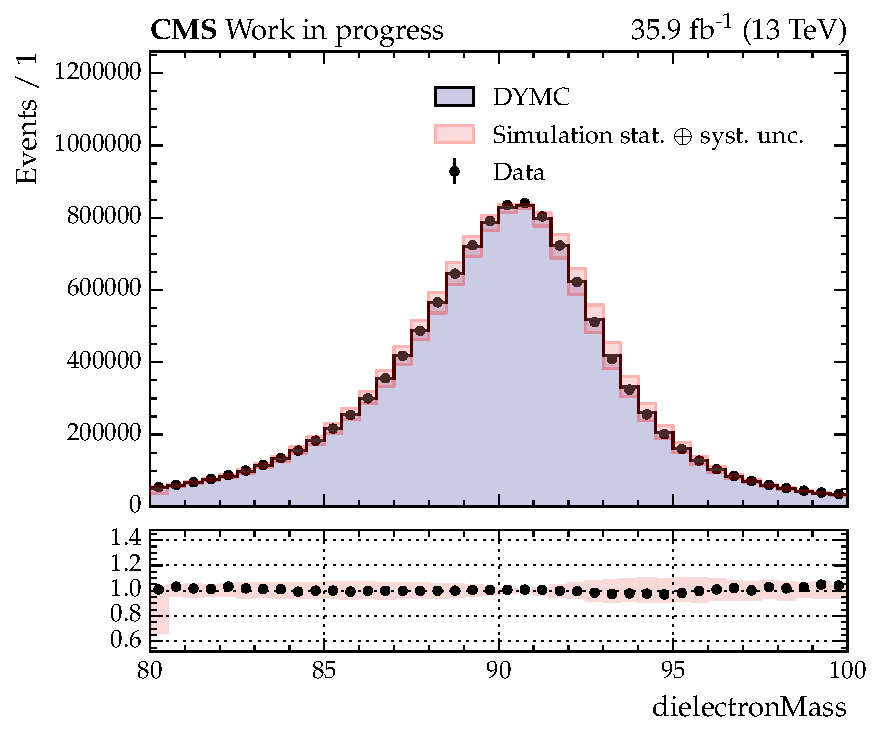
\includegraphics[width =0.46\linewidth]{Figures/Hee/simulationCorrections/DY/DY_validation_ggH_BDT_dielectronMass_2016.pdf}\hfill%
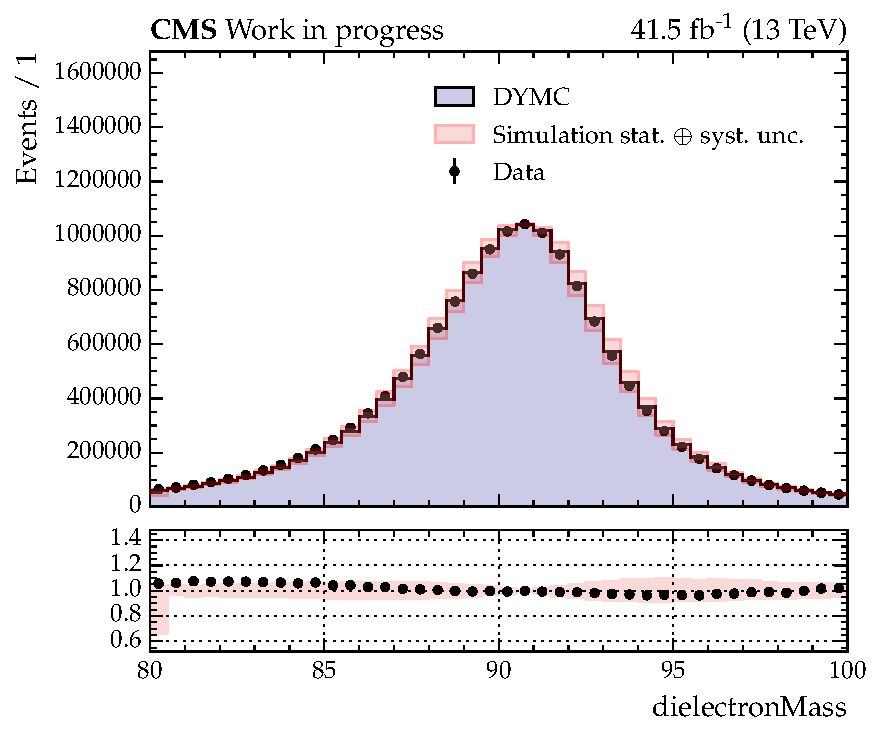
\includegraphics[width =0.46\linewidth]{Figures/Hee/simulationCorrections/DY/DY_validation_ggH_BDT_dielectronMass_2017.pdf}\hfill\\%
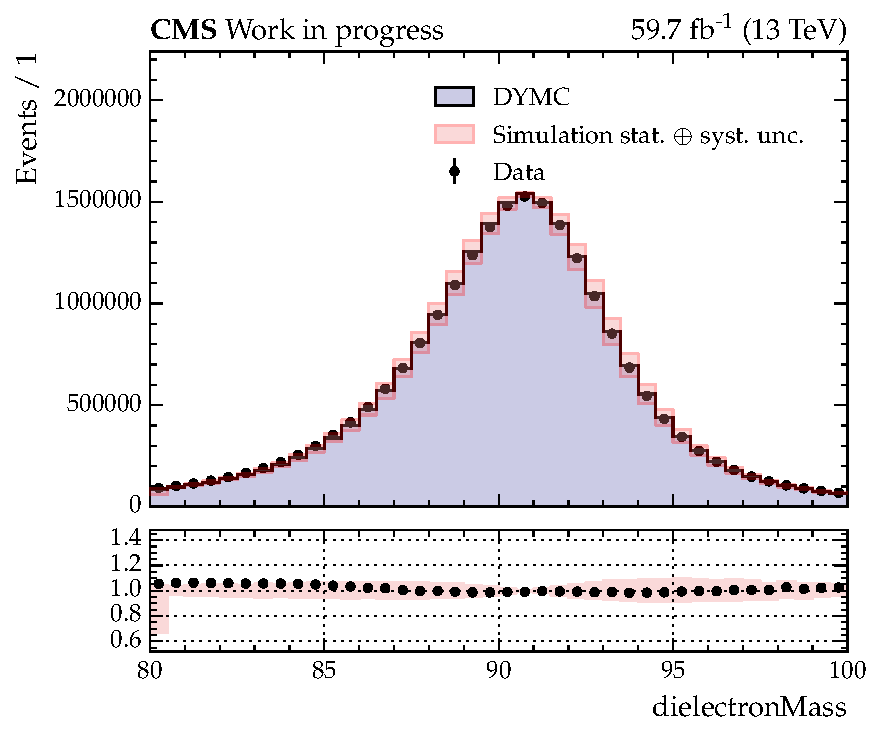
\includegraphics[width =0.46\linewidth]{Figures/Hee/simulationCorrections/DY/DY_validation_ggH_BDT_dielectronMass_2018.pdf}\hfill%
\caption[Dielectron invariant mass distributions for \Zee events in the \Hee control region.]{The dielectron invariant mass distribution for \Zee events in the \Hee control region, compared between data and simulation following the electron energy scale and resolution corrections. The control region is defined identically to the analysis preselection, with the exception of the dielectron mass requirements, which are shifted to $80<\mee<100$~GeV. The red band indicates the combination of statistical and systematic uncertainties for simulated \Zee events, where the systematic component comprises the uncertainty on the electron energy scale corrections. The agreement between data and simulation is within the combined uncertainty from statistical and systematic sources, for each year independently.} 
\label{fig:hee_mee_scales_smearings}            
\end{figure}

\subsubsection{Final electron energy and resolution}

The final electron energy is obtained from a combination of the ECAL energy, the GSF track momentum, and all associated energy deposits from bremsstrahlung photons and electron-positron pairs identified by the conversion finding algorithm. 
%charge mis-assignment is 0.1\% in barrel and 0.3\% in endcap - got from track curvature (3 independent checks)
The energy resolution is measured using electrons from \Zee decays. Appendix~\ref{app:electron_enenergy_scale_corr} shows the cumulative impact of the electron reconstruction process, including application of the electron energy scale and resolution corrections. The performance as a function of electron $|\eta|$ is shown for each year in the Run 2 campaign in Figure~\ref{fig:cms_energy_res_vs_eta}~\cite{Run2_ECAL_plots,CMS_egamma_performance}. The resolution is extracted for all electrons inclusively, and independently for low bremsstrahlung electrons, defined by a minimum requirement on the $R_{9}$ quantity. In the latter regime, the momentum resolution for electrons is around 1.6\% for those in the barrel, rising to values of around 5\% in the endcaps, where the effect of an increased upstream material budget is more evident. Inclusively, the energy resolution varies between 2 to 4\% in the barrel, and worsens to around 4 to 5\% in the endcaps. The radiation damage sustained to ECAL crystals during the LHC operation results in a small worsening of the resolution with year; however, the overall performance during Run 2 is stable, despite the increased luminosity and material degradation. 


\begin{figure}[htbp!]
\centering
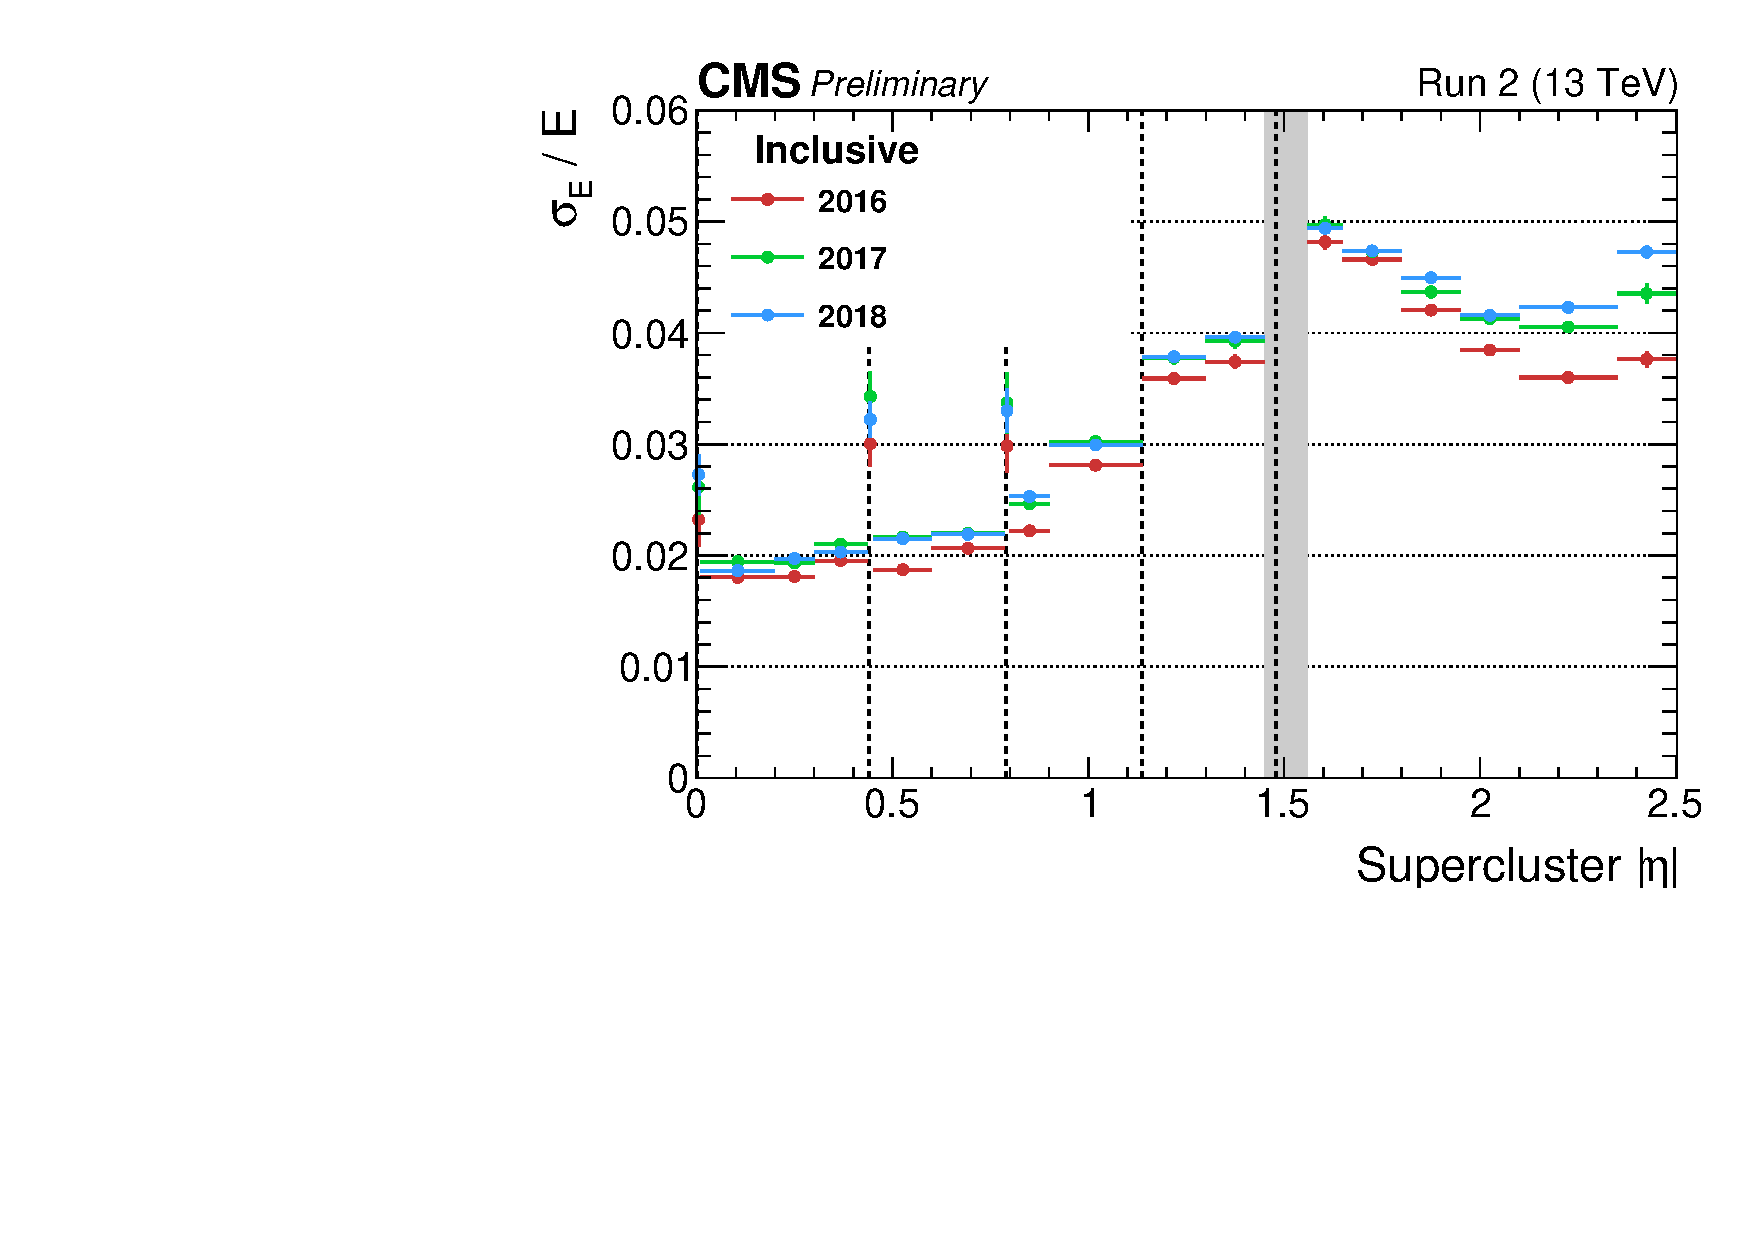
\includegraphics[width =0.49\linewidth]{Figures/Detector/CMS/energy_res_vs_eta_inc.pdf}\hfill%
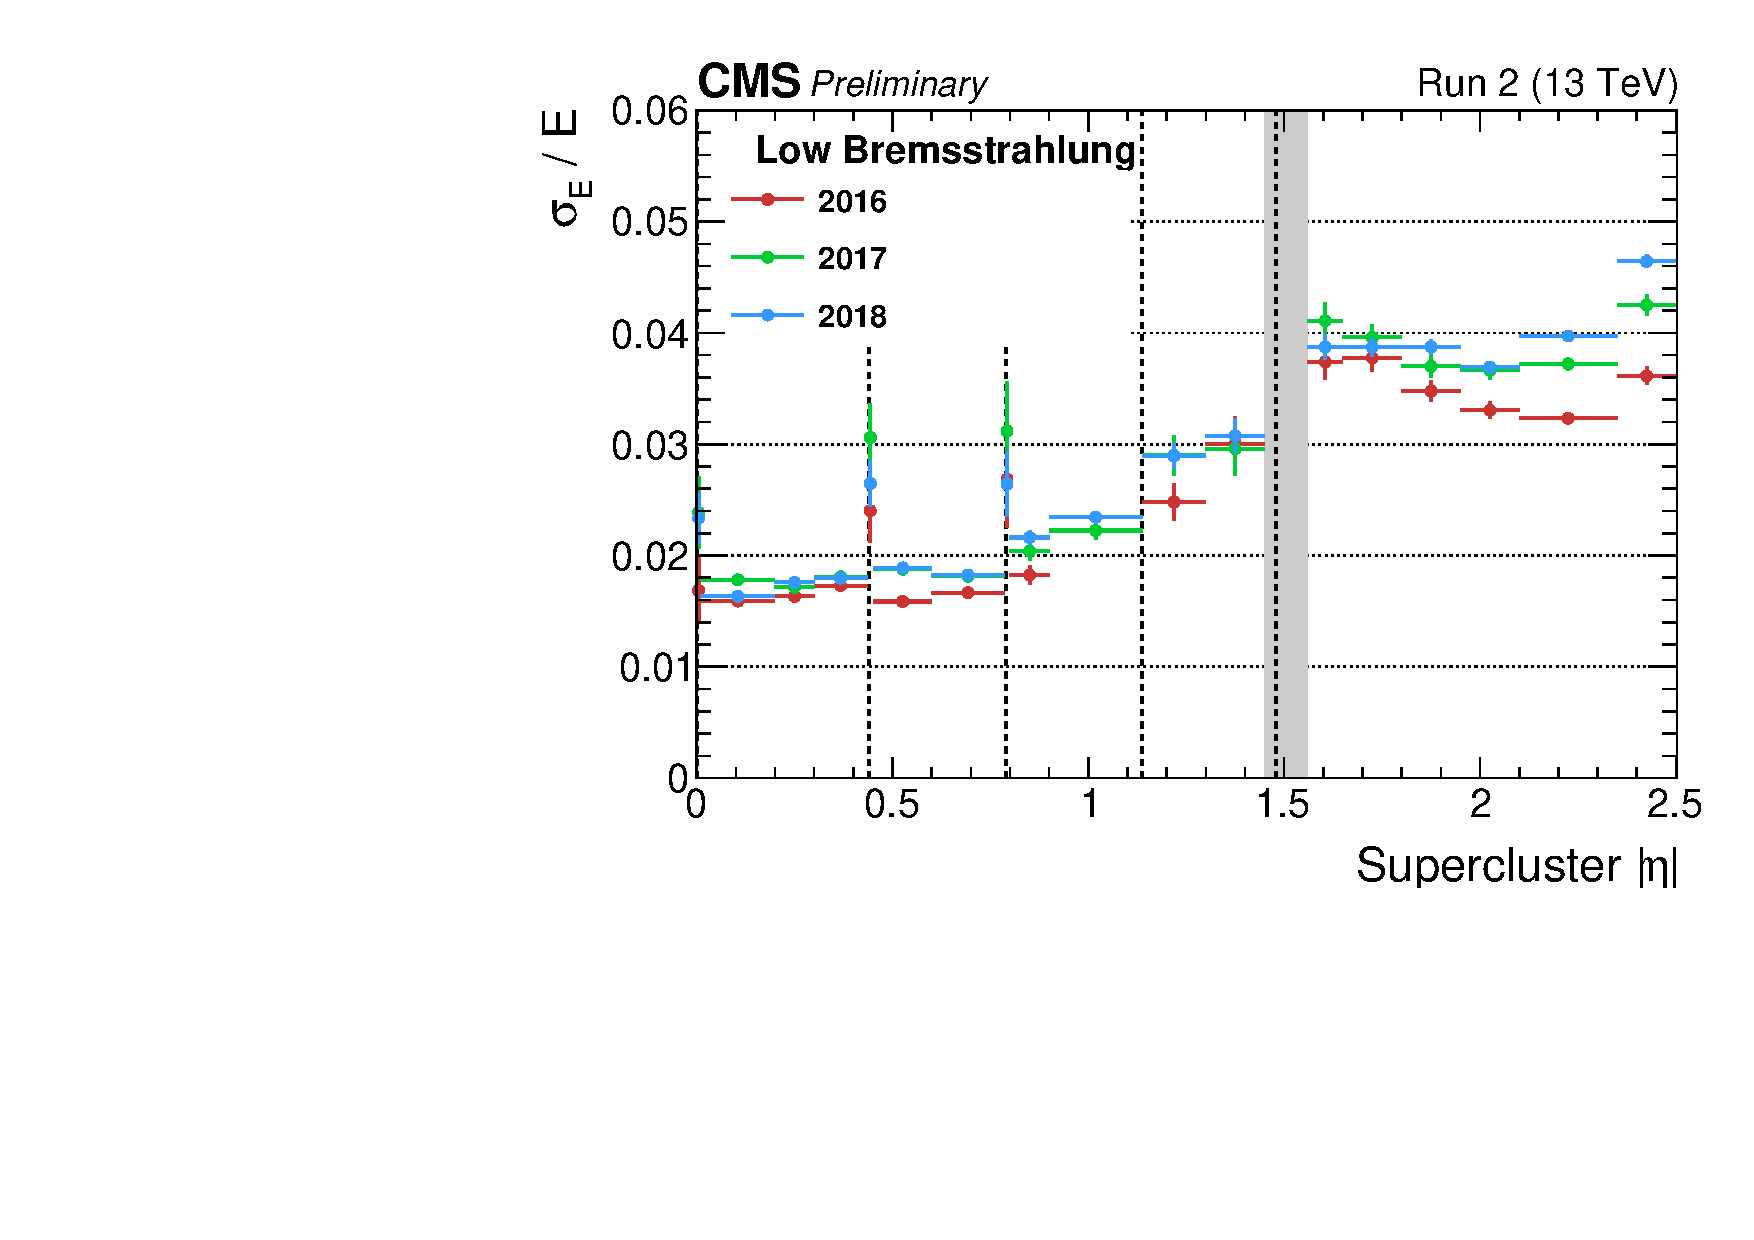
\includegraphics[width =0.49\linewidth]{Figures/Detector/CMS/energy_res_vs_eta_low_brem.pdf}\hfill
\caption[The relative energy resolution for electrons from \Zee decays.]{The relative energy resolution for electrons from \Zee decays, for each year of data taking during Run 2 operation, shown as a function of electron $|\eta|$. The transition region between the ECAL barrel and endcap ($1.44<|\eta|\;<1.57$) is shaded grey. Left: the inclusive performance shown for all electrons. Right: the performance evaluated in a low electron bremsstrahlung regime, defined by $R_{9}>0.94$.
The resolution is extracted from a likelihood fit to the \mee distribution, using a Breit-Wigner convolved with a Gaussian function as the \Zee signal model. Figures taken from Ref~\cite{Run2_ECAL_plots}.} %continuum background component is also modelled
\label{fig:cms_energy_res_vs_eta}                                              
\end{figure}

%calibration using cosmics, test beams etc: https://arxiv.org/pdf/1706.04965.pdf

\subsection{Photons}

Photon reconstruction is performed separately for isolated and non-isolated photons. Since the basic properties and energy deposition patterns of isolated photons are similar to electrons, their reconstruction within the PF framework is performed together. These photons are formed from ECAL clusters with $E_{T}$ above 10~GeV that are well isolated from tracks and calorimeter clusters, and have no link to a GSF track. A selection is also placed on quantities that describe photon energy deposit patterns, such as the ratio of energy clustered in the HCAL to that in the ECAL.

Non-isolated photons are typically found within hadronic jets, most notably from the $\pi^{0}\rightarrow\gamma\gamma$ meson decay. These are formed using ECAL clusters not linked to tracks, provided the photon was reconstructed within the tracker acceptance. The preference for identifying ECAL deposits with photons over neutral hadrons is justified by the observation that in hadronic jets, 25\% of the energy is carried by photons, while neutral hadrons only deposit 3\% of their energy. Beyond the tracker acceptance however, the presence of charged hadrons adds additional ambiguity, and the preference given to photons is no longer justified. Therefore, reconstruction in this region asserts that ECAL clusters resulting from photon interactions are not linked to any HCAL clusters.

The final energy measurement is taken from the SC deposits in the calorimeter systems. This includes the energy of all associated electron pairs resulting from conversions (and associated bremsstrahlung photons), which is particularly important since the fraction of conversions occurring before the last tracker layer can be as high as 60\% for regions with the largest amount of tracker material in front of the ECAL~\cite{CMS_egamma_performance}. Once the energy scale and resolution are corrected in the procedure described above, the energy resolution of photons is around 1--2.5\% in the barrel, which degrades to approximately 2.5\%--4\% in the endcaps~\cite{photon_conversion_finder,Run2_ECAL_plots}.

\subsection{Muons}

Tracks resulting from muons are reconstructed independently in the inner tracker and muon systems~\cite{muon_reco}. Hits within DT or CSC detector systems are used to form track segments. The segments seed track fits which also use information from the RPCs, forming \textit{standalone} muon tracks. Association of standalone tracks to those in the inner tracker results in one of two different muon types being reconstructed:

\begin{itemize}
    \item \textit{Tracker muon:} unique inner tracks are extrapolated to the muon system, and are compatible with one standalone muon track segment.
    \item \textit{Global muon:} standalone muon tracks are matched to tracks in the inner tracker. 
\end{itemize}

\noindent At low \pt, the reconstruction is driven by tracker muons, since such muons rarely penetrate multiple components in the muon system. Conversely, global muons drive the reconstruction of muons with high \pt, where the tracker-only fit is poor. The momentum resolution for muons is around 1\% (3\%) in the barrel (endcaps) for muons with $\pt<100$~GeV. This resolution degrades significantly for high \pt muons; in the barrel region, muons with \pt up to 1~TeV achieve a momentum resolution of around 7\%.

\subsection{Hadrons}
\label{subsec:hadrons_and_jets}

At this stage, only charged hadrons including $\pi^{\pm}$, $K^{\pm}$, and protons, and neutral hadrons such a $K^{0}$ and neutrons, remain to be identified. In practise, these are considered in the same processing step as non-isolated photons, described earlier. Within the tracker acceptance, all HCAL reconstructed clusters not linked to tracks are identified as neutral hadrons. The situation is complicated outside of the tracker acceptance where charged and neutral hadrons cannot be separated. Instead, ECAL clusters that are also linked to clusters in the HCAL are assigned to either charged or neutral hadron showers.

\subsubsection{Jets}


Particles produced from the hadronisation of quarks or gluons are collected into collimated sprays known as jets. The clustering at CMS is performed using the anti-$k_{t}$~\cite{anti-kt} jet finding algorithm, which groups PF candidates into conical clusters. Typical jet finding algorithms define a distance metric between constituent particles; in the anti-$k_{t}$ algorithm, this metric is formed in an abstract space of momentum, rapidity, and azimuthal angle. Clustering starts with the two objects that are nearest in distance and repeats iteratively until the shortest distance is between an object and the beampipe. At this point, the resulting jet is removed from consideration and the process may begin again.
%infrared safe or soft emission safe: add soft emmisions process and have it unchanged (ME not blowing up)
% collinear safe: ME doesn't blow up when massless particle produce colllinearly from another
    
The PF candidates considered during jet finding are subject to a charged hadron subtraction procedure (CHS), designed to reduce jet contributions resulting from pileup. The CHS procedure identifies the vertex for each charged PF candidate, removing those which are unambiguously associated with pileup vertices. Since the CHS procedure requires tracking information to identify PU vertices, only jets within $|\eta|\;<2.5$ are subject to this correction. For jets within the tracker acceptance, CHS removes approximately 50\% of pileup clusters.

Although CHS removes a significant fraction of PU, additional corrections are applied to specifically reduce PU contributions to jet energy and momenta. The correction factors are differential in quantities sensitive to pileup, including $\eta$, \pt, average event energy density, and jet area. Following these corrections, the jet energy scale and resolution is corrected in both data and simulation~\cite{JESAndJERCorrections}. These corrections are derived in bins of \pt and $\eta$, resulting in agreement within 0.5\% of the generator-level jet energy over a wide range of momenta. Finally, any residual differences between data and simulation are corrected using dijet and single jet events in samples of $\mathrm{Z}(\rightarrow\mu\mu)$+jet, $\mathrm{Z}(\rightarrow\mathrm{ee})$+jet, $\gamma$+jet, and multi-jet events. These corrections exploit the transverse momentum balance between the jet to be calibrated and a well-measured reference object, to correct for jet energy scales deviating from unity. Following these sets of corrections, the jet energy resolution ranges between approximately 15 to 20\% at 30~GeV, 10\% at 100~GeV, and 5\% at 1~TeV~\cite{JESAndJERCorrections}.

\subsection{Missing transverse momentum}
\label{subsec:mpt}


The presence of particles that do not interact with the detector material, notably neutrinos, can be inferred from a \pt imbalance in an event, referred to as missing transverse momentum. This is defined as the negative vector sum of the transverse momenta of all PF candidates in an event, $p_{T}^{\mathrm{miss}}$. The reconstruction of $p_{T}^{\mathrm{miss}}$ relies heavily on the hermeticity of the detector, and maintaining low misidentification and misreconstruction efficiencies for physics objects that could fake $p_{T}^{\mathrm{miss}}$.


\section{Summary}

Particle reconstruction at the CMS detector optimally combines information from each subdetector, in a technique known as particle flow. This results in a set of physics objects available for analysis, including electrons, photons, hadrons, and muons. The reconstruction of many objects includes a set of dedicated corrections; for electrons, these are designed to improve agreement between simulation and data, and the dielectron mass (resolution), which is later fit to extract the analysis' results. These corrections, which are similar for electron and photon objects, proceed via a multi-step regression which uses descriptions of the supercluster profile and track-related quantities as inputs. The reconstruction of electrons also uses an identification criterion designed to reduce contamination from objects that could fake prompt electrons. Further selection is applied to other objects used within the \Hee search, including jets, where the requirements aim to reduce contamination from pileup clusters. 
%Corrections are then applied to the jet energy scale and resolution in both simulation and data.




